\documentclass{article}
\usepackage[utf8]{inputenc}


\usepackage[lined, boxed, linesnumbered]{algorithm2e}
\usepackage{natbib}
\usepackage{amsfonts}
\usepackage{amsthm}
\usepackage{float}
\usepackage{mathtools}
\usepackage{graphicx}
\usepackage{multicol}
\usepackage{blindtext}
\usepackage[top=2cm, bottom=2cm, left=2cm, right=2cm]{geometry}
\usepackage{fancyhdr}

\bibliographystyle{apalike}

\newtheorem{theorem}{Theorem}[section]
\newtheorem{corollary}{Corollary}[theorem]
\newtheorem{lemma}[theorem]{Lemma}


%%%%%%%%%%%%%%%%%%%%%%%%%%%%%% FANCY HEADER %%%%%%%%%%%%%%%%%%%%%%%%%%%%%%%%%%%
\fancyhead{}
\fancyfoot{}
\fancyhead[C]{\bf Resource constrained scheduling: a temporal networks approach}
\renewcommand{\headrulewidth}{1pt}
\newcommand{\HRule}{\rule{\linewidth}{0.5mm}}

%%%%%%%%%%%%%%%%%%%%%%%%%%%%%% DOCUMENT %%%%%%%%%%%%%%%%%%%%%%%%%%%%%%%%%%%%%%%

\begin{document}
\thispagestyle{empty}

\begin{center}
%%%%%%%%%%%%%%%%%%%%%%%%%%%%%% TITLE PAGE %%%%%%%%%%%%%%%%%%%%%%%%%%%%%%%%%%%%%
\HRule \\[0.3cm]
{\Large \bfseries
Temporal Networks with Resource Constraints\\[0.3cm]}
\HRule \\[0.5cm]

\noindent
\begin{minipage}{0.5\textwidth}
\begin{flushleft}
\textbf{Szymon Sidor\\
Brian Williams}\\
Massachusetts Institute of Technology
\end{flushleft}
\end{minipage}%
\begin{minipage}{0.5\textwidth}
\begin{flushright}
\textsc{sidor@mit.edu}\\
\textsc{williams@mit.edu}\\
$\ $
\end{flushright}
\end{minipage}
\\[1cm]
\end{center}
\pagestyle{fancy}

\begin{multicols}{2}
%%%%%%%%%%%%%%%%%%%%%%%%%%%%%% ABSTRACT %%%%%%%%%%%%%%%%%%%%%%%%%%%%%%%%%%%%%%%
\begin{abstract}
\noindent TODO
\end{abstract}
%%%%%%%%%%%%%%%%%%%%%%%%%%%%%% INTRODUCTION %%%%%%%%%%%%%%%%%%%%%%%%%%%%%%%%%%%
\section{Introduction}
TODO
%%%%%%%%%%%%%%%%%%%%%%%%%%%%%% RELATED WORK %%%%%%%%%%%%%%%%%%%%%%%%%%%%%%%%%%%
\section{Related Work}
%\blindtext[5]

One of the earliest mentions of a scheduling problem being solved in an algorithmic fashion can be found in \cite{johnson1954optimal}, although there's evidence that the problem was already considered in unpublished versions of \cite{bellman1956mathematical}. This publication considers the following statement of scheduling problem. We have $n$ items and $m$ stages and $A_{i,j}$ denoting the time for $i$-th item to be processed by stage $j$. All the items must be processed by different stages in order (for example first stage is printing of a book and second stage is binding). The publication considers $m=2$ and $m=3$ and arrives at the solution that \textit{``permits one to optimally arrange twenty production items in about five minutes by visual inspection''}. It turns out that the solution to the problem for $m \geq 3$ is NP-hard (\cite{garey1976complexity}). In \cite{wagner1959integer} an Integer Programming solution to the scheduling problem and noticed that it \textit{``is a single model which encompasses a wide variety of machine-scheduling situations''}.

In \cite{pritsker1969multiproject} a generalization of scheduling problem is considered, which allows for multiple resource constraints. However the solution provided uses a discrete time formulation, which depending on required accuracy can substantially decrease performance. Work in this publication considers work on Temporal Networks, which explicitly model continuous time constraints. Interestingly, one of the publications about resource constrained scheduling (\cite{bartusch1988scheduling}) used the notion of which can be thought of as resource constrained scheduling over Simple Temporal Networks (STN). The publication derives the theory behind STNs 3 years before the STN publication!

In \cite{dechter1991temporal} a notion of Simple Temporal Problem was introduced which allows one to solve problem with simple temporal constraints of form $l \leq t_y - t_x \leq u$. This simple concept was later extended with various more sophisticated notions of temporal constraints. \cite{vidal1996dealing} defined the notion of uncertain temporal constraint, where the duration between two time events can take a value from an interval $[l,u]$ which is unknown during the time of scheduling (uncertain duration constraints); consistency of such temporal networks is called Strong Controllability. \cite{morris2001dynamic} desribes a pseudopolynamial algorithm for handling uncertain duration constraint, where we are allowed to make a descition scheduling decitions based on knowledge of uncertain durtions from the past (Dynamic controllability). His algorithm is later improved to polynamial complexity (\cite{morris2005temporal}). Finally, \cite{Fang2014} provides a non-linear optimization based solver for uncertain temporal constraints where the duration of the constraint can come from abritrary probabilistic distribution.

%%%%%%%%%%%%%%%%%%%%%%%%%%%%%% PROBLEM STATEMENT %%%%%%%%%%%%%%%%%%%%%%%%%%%%%%
\section{Problem statement}
In this section we will define notion of a Time Resource Network (TRN) and the relevant constraint on TRN's schedule - Resource Consistency. All the results presented in this paper can be extended to multiple different type of resources being constrained at the same time (electricity, water, fuel, cpu time, memory etc.), but to simplify the notation we will assume that only one type of resource is constrained. Additionally, for simplicity we only consider the problem of consistency, but the techniques presented in this paper can be easily extended to objective optimization over constrained schedules.
\subsection{Abstract Temporal Network}
Since TRNs can operate on top of many different types of temporal networks, we define a notion of Abstract Temporal Network (ATN), to capture only the necessary properties. For abstract temporal network we define two pieces of functionality:
\begin{enumerate}
\item \texttt{nodes(ATN)}, which returns a set of timepoints in $ATN$
\item \texttt{extend(ATN, $\{ stc_1, ... stc_n \} $)}, which takes ATN and a set of simple temporal constraints (\cite{dechter1991temporal}) spanning \texttt{nodes(ATN)}, and returns another $ATN'$, such that there exists a schedule satisfying $TC(ATN')$ if and only if there exists a schedule satisfying $TC(ATN)$ and the obeying set of simple temporal constraint $\{ stc_1, ... stc_n \} $. $TC$ is a notion of probabilistic temporal consistency described in section \ref{temporal_consistency}.
\end{enumerate}
As the following section describes in detail we will use \texttt{extend} to encode resource constraints over \texttt{nodes}.
\subsection{Schedule}
A schedule $s: \texttt{nodes(ATN)} \rightarrow \mathbb{R}$ is a mapping from abstract time points in ATN to concrete execution times.
\subsection{Temporal Consistency}
\label{temporal_consistency}
For an ATN we define a predicate $TC_s(ATN)$, which means that $ATN$ is \textbf{temporally consistent} under schedule $s$. $TC_s$ is true if schedule $s$ satisfies all the constraints of the $ATN$ (what that means precisely depends on the $ATN$ - we only require for it to be verifiable). We say that that $TC(ATN)$ which means that there exists at schedule $s$ such that $TC_s(ATN)$.
\paragraph{Example}
Example network that satisfies the ATN interface is Simple Temporal Network with Uncertainty (STNU) described in \cite{vidal1996dealing}. Let $N$ be an STNU. Using the terminology from the paper \texttt{nodes($N$)} is the set of received and activated nodes and \texttt{extend($N$, $\{ stc_1, ... stc_n \} $)} augments $N$ with $stc_i$ encoded as a controllable link. One way to define is $TC(N)$ is to be true if and only if $N$ is strongly controllable.
%Let's consider cc-pSTP \cite{Fang2014} as an example. Here \texttt{nodes} returns set of \textit{activated} and \textit{received} timepoints. \texttt{extend} returns network with extra \textit{free contraints} encoding the simple temporal constraints. The temporal consistency check $TC$ is true if cc-pSTP has a solution.
\subsection{Time Resource Network}
\label{sec:trn_definition}
A Time Resource Network is described by a tuple $TRN = (ATN, R)$, where $ATN$ is an Abstract Temporal Network and $R={src_1, ..., src_n}$ is a set of \textbf{simple resource constraints}, each of which is a triplet $(x, y, r)$, where $x, y \in$ \texttt{nodes(ATN)} and $r \in \mathbb{R}$ is resource usage which can be positive (consumption) and negative (generation). Given a schedule $s$ for any time $t \in \mathbb{R}$ resource \textbf{usage} for that simple resource constraint $src=(x,y,r)$ is equal to
\begin{align*}
u_s(src, t) = \begin{cases}
r & \text{if}\ s(x) \leq t \leq s(y)\\
0 & \text{otherwise}
\end{cases}
\end{align*}
Intuitively, simple resource constraint encodes the fact that between time $s(x)$ and $s(y)$  resource is consumed (generated) at the rate $|r|$ units of resource per unit time for positive (negative) $r$.

Our notation is inspired by \cite{bartusch1988scheduling}. In particular notice that one can encode arbitrary piecewise-constant resource profile, by decomposing it into simple resource constraint expressing usages at every constant intervals and simple temporal constraints joining their ends (details can be found in \cite{bartusch1988scheduling}).


\subsection{Resource consistency}
For a schedule $s$ we define a \textbf{net-usage} at time $t \in \mathbb{R}$ as $U_s(t)$ in the following way:
\[
U_s(t) = \sum_{\forall_{src_i \in R}} u_s(src_i, t)
\]
Where $R$ is a set of all the resource constraints and. We say that the network is \textbf{resource consistent} under schedule $s$ when it satisfies predicate $RC_s(TRN)$, i.e.
\[
\forall_{t} . U_s(t) \leq 0
\]
Intuitively it means that resource is never consumed at a rate which is greater than the generation rate. We say that $TRN$ is resource consistent is there exists $s$ such that $RC_s(TRN)$.
\subsection{Time-resource consistency}
$TRN=(ATN, R)$ is \textbf{time-resource consistent} if there exists a schedule $s$ such that $RC_s(TRN) \wedge TC_s(ATN)$. Determining whether a $TRN$ is time-resource consistent is the central problem tackled in this publication.

\subsection{Properties of TRN}
Before we proceed to describe algorithms for determining time-resource consistency it will be helpful to understand some properties that apply to every TRN.
\begin{lemma}
\label{resource_checking}
Assume we have a TRN, such that ATN has explicit timepoints for start and end of the time horizon (can be $\pm \infty$).
A schedule is resource-consistent if and only if
\begin{align}
\label{eq:resource_consistency}\forall_{t \in \texttt{nodes(ATN)}} U_s(s(t)) \leq 0
\end{align}
i.e. resource usage is not non-positive at all of the scheduled timepoints.
\end{lemma}
\begin{proof}
$\Rightarrow$ Trivial from definition of resource-consistency.
$\Leftarrow$ We say a time $t \in \mathbb{R}$ is scheduled if there exists a timepoint  $x \in \texttt{nodes(ATN)}$ such that $t = s(x)$. We can rephrase right side of the lemma saying that for all the scheduled $t$ $U_s(t) \leq 0$. Assume that the right side of the implication is satisfied but the schedule is not resource consistent. That means that there exists a time point $t_{danger}$ which is not schduled for which $U_s(t_{danger}) > 0 $. Let $x$ be highest scheduled time less than $t_{danger}$ and let $y$ be smallest scheduled time higher than $t_{danger}$. We know that $U_s(t)$ for $x \leq t \leq y$ is a sum of linear functions (or possibly zero), which is itself a linear function. This means that either $U_s(x) \geq t_{danger}$ or $U_s(y) \geq t_{danger}$, so either $U_s(x) > 0$ or $U_s(y) > 0$. But both $x$ and $y$ are scheduled. Contradiction.

\end{proof}
\begin{corollary}
Given a $TRN$ with only simple resource constraints and two schedules $A$ and $B$ that have the same ordering of timepoints, $A$ is $p$-resource-consistent if and only if $B$ is $p$-resource-consistent.
\end{corollary}
\begin{proof}
Notice that if we move arbitrary timepoint, while preserving the relative ordering of timepoints, then net resource usage at that timepoint will not change (as the $U_s(t)$ between the neighboring timepoints remains constant). Therefore by lemma \ref{resource_checking} we can transform schedule $A$ into schedule $B$.
\end{proof}
Notice that the Corollary does not apply to the linear resource constraints (see fig. TODO).

TODO: generalize to probabilistic

Finally we say that a TRN is \textbf{$p$-time-resource consistent} if there exists and ordering of timepoints such that every schedule that satisfies this ordering is $p$-resource-consistent and $ATN$ extended with that ordering is $TC$.

\subsection{Common scheduling problems expressed as Time Resource Network}

\subsection{Going beyond schedules}
TODO: execution strategies

%%%%%%%%%%%%%%%%%%%%%%%%%%%%%% ALGORITHM %%%%%%%%%%%%%%%%%%%%%%%%%%%%%%%%%%%%%%
\section{Approach}
In this section be present two alternative approaches to solving the problem. One of them is using Mixed Integer Programming (MIP) and the other is using Constraint Satisfaction Problem (CSP) formulations.
\subsection{Mixed Integer Programming based algorithm}
Mixed Integer Programming (\cite{markowitz1957solution}) is a very natural way of expressing scheduling problems. It's flexibility and efficiency causes many researchers to choose this method to tackle scheduling problems. In this section we present a way to formulate TRN as a MIP problem. Let's take a $TRN=(ATN, R)$ where $R={src_1, ..., src_n}$ and $src_i = (x_i, y_i, r_i)$ as defined in section \ref{sec:trn_definition}. Let $TC-fromulation(ATN)$ be a MIP-formulation that is consistent if an only if $TC(ATN)$. For some types of $ATN$ such a formulation might not exist and in those cases MIP-based algorithm cannot be applied. To help use define the MIP-formulation concisely let's introduce resource-change at timepoint $n$ as:
\begin{align*}
\Delta(n) = \sum_{(x_i, y_i, r_i) \in R, x_i = n} r_i + \sum_{(x_i, y_i, r_i) \in R, y_i = n} -r_i
\end{align*}
Also let's denote all the timepoints relevant for resource constraints as $RT \subseteq nodes(ATN)$, i.e.
\begin{align*}
RT = \{ x_i | (x_i, y_i, r_i) \in R \} \cup \{ y_i | (x_i, y_i, r_i) \in R \}
\end{align*}
Intuitively $\Delta(n)$ is the amount by which resource usage changes after time $s(n)$ under schedule $s$.

We propose the following formulation:
\begin{align}
\label{eq:mip0} & \forall_{t \in nodes(ATN)}.              & 0 \leq t \leq M \\
\label{eq:mip1} & \forall_{t_1, t_2 \in RT, t_1 \neq t_2}. & t_1 - t_2 \geq - x_{t_1,t_2} M \\
\label{eq:mip2} & \forall_{t_1, t_2 \in RT, t_1 \neq t_2}. & t_1 - t_2 \leq (1.0 - x_{t_1,t_2}) M\\
\label{eq:mip3} & \forall_{t_1, t_2 \in RT, t_1 \neq t_2}. & x_{t_1,t_2} + x_{t_2,t_1}  = 1\\
\label{eq:mip4} & \forall_{t_1, t_2 \in RT, t_1 \neq t_2}. & x_{t_1,t_2} \in \{ 0, 1 \} \\
\label{eq:mip5} & \forall_{t_1 \in RT}.                    & \sum_{t_2 \in RT} x_{t_2, t_1} \Delta(t_2) \leq 0\\
\label{eq:mip6} & \text{TC-fromulation(ATN)}
\end{align}

Variable $M$ denotes the time horizon, such that all the variables are scheduled between $0$ and $M$. This definition is imposed in eq. \ref{eq:mip0}.
Variables $x_{t_1,t_2}$ are order variables, i.e.
\begin{align*}
x_{t_1, t_2} = \begin{cases}
1 &\text{ if }s(t_1) \leq s(t_2) \\
0 &\text{ otherwise}
\end{cases}
\end{align*}
Equations \ref{eq:mip1}, \ref{eq:mip2}, \ref{eq:mip3}, \ref{eq:mip4} enforce that definition. In particular equations \ref{eq:mip1}, \ref{eq:mip2} enforce the ordering using big-$M$ formulation that is correct because of time horizon constraint. In theory eq. \ref{eq:mip3} could be eliminated by careful use of $\epsilon$ (making sure no two timepoints are scheduled at exactly the same time), but we found that in practice they result in useful cutting planes that decrease the total runtime. Equation \ref{eq:mip5} ensures resource consistency by lemma \ref{resource_checking}. Finally eq. \ref{eq:mip6} ensures time consistency.

\subsection{Constraint Satisfaction Programming based algorithm}
High level idea of the algorithm is quite simple and is presented in algorithm \ref{hl_algo}. In the second line we iterate over all the permutations of the timepoints. On line 3 we use \texttt{p\_resource\_consistent} function to check resource consistency, performing this check is the nontrivial part of the algorithm. On line four we use $TC$ checker to determine if network is time consistent - the implementation depends on $ATN$ and we assume it is available. Function $encode\_as\_scts$ encodes permutation using simple temporal constraints. For example if $\sigma(1) = 2$ and $\sigma(2) = 1$ and $\sigma(3) = 3$, then we can encode it by two STCs: $ 2 \leftarrow 1 $ and $1 \leftarrow 3$.

\begin{algorithm}[H]
    \label{hl_algo}
    \KwData{TRN and p}
    \KwResult{true if TRN=(ATN, RC) is p-time-resource-consistent}
    $N \leftarrow \texttt{nodes(ATN)}$\;
    \For{$\sigma \leftarrow \text{permutation of } N$}{
        \If{\texttt{p\_resource\_consistent(RC, $\sigma$, $p$)} }{
            \If{TC(\texttt{extend(ATN, encode\_as\_scts($\sigma$))})}{
                succeed\;
            }
        }
    }
    fail\;
    \caption{Checking $p$-time-resource-consistency of a TRN }
\end{algorithm}
Implementation of \texttt{p\_resource\_consistent} follows from lemma \ref{resource_checking}.



% INPUT: atn N, {src} S (spanning N.timepoints)
% OUTPUT: scheduling strategy on N or fail
% ALGORITHM:
% X = subset of N.timepoints used by SRCs from S
% for every permutation pi of X:
% stcs = pi encoded by STCs
% result = N.solve_with_stcs(stcs)
% if result is schedule:
%        return schedule
%       fail



%%%%%%%%%%%%%%%%%%%%%%%%%%%%%% EXPERIMENTS %%%%%%%%%%%%%%%%%%%%%%%%%%%%%%%%%%%%
\section{Experiments}
\subsection{TRN over STN}

\begin{figure*}
\begin{center}
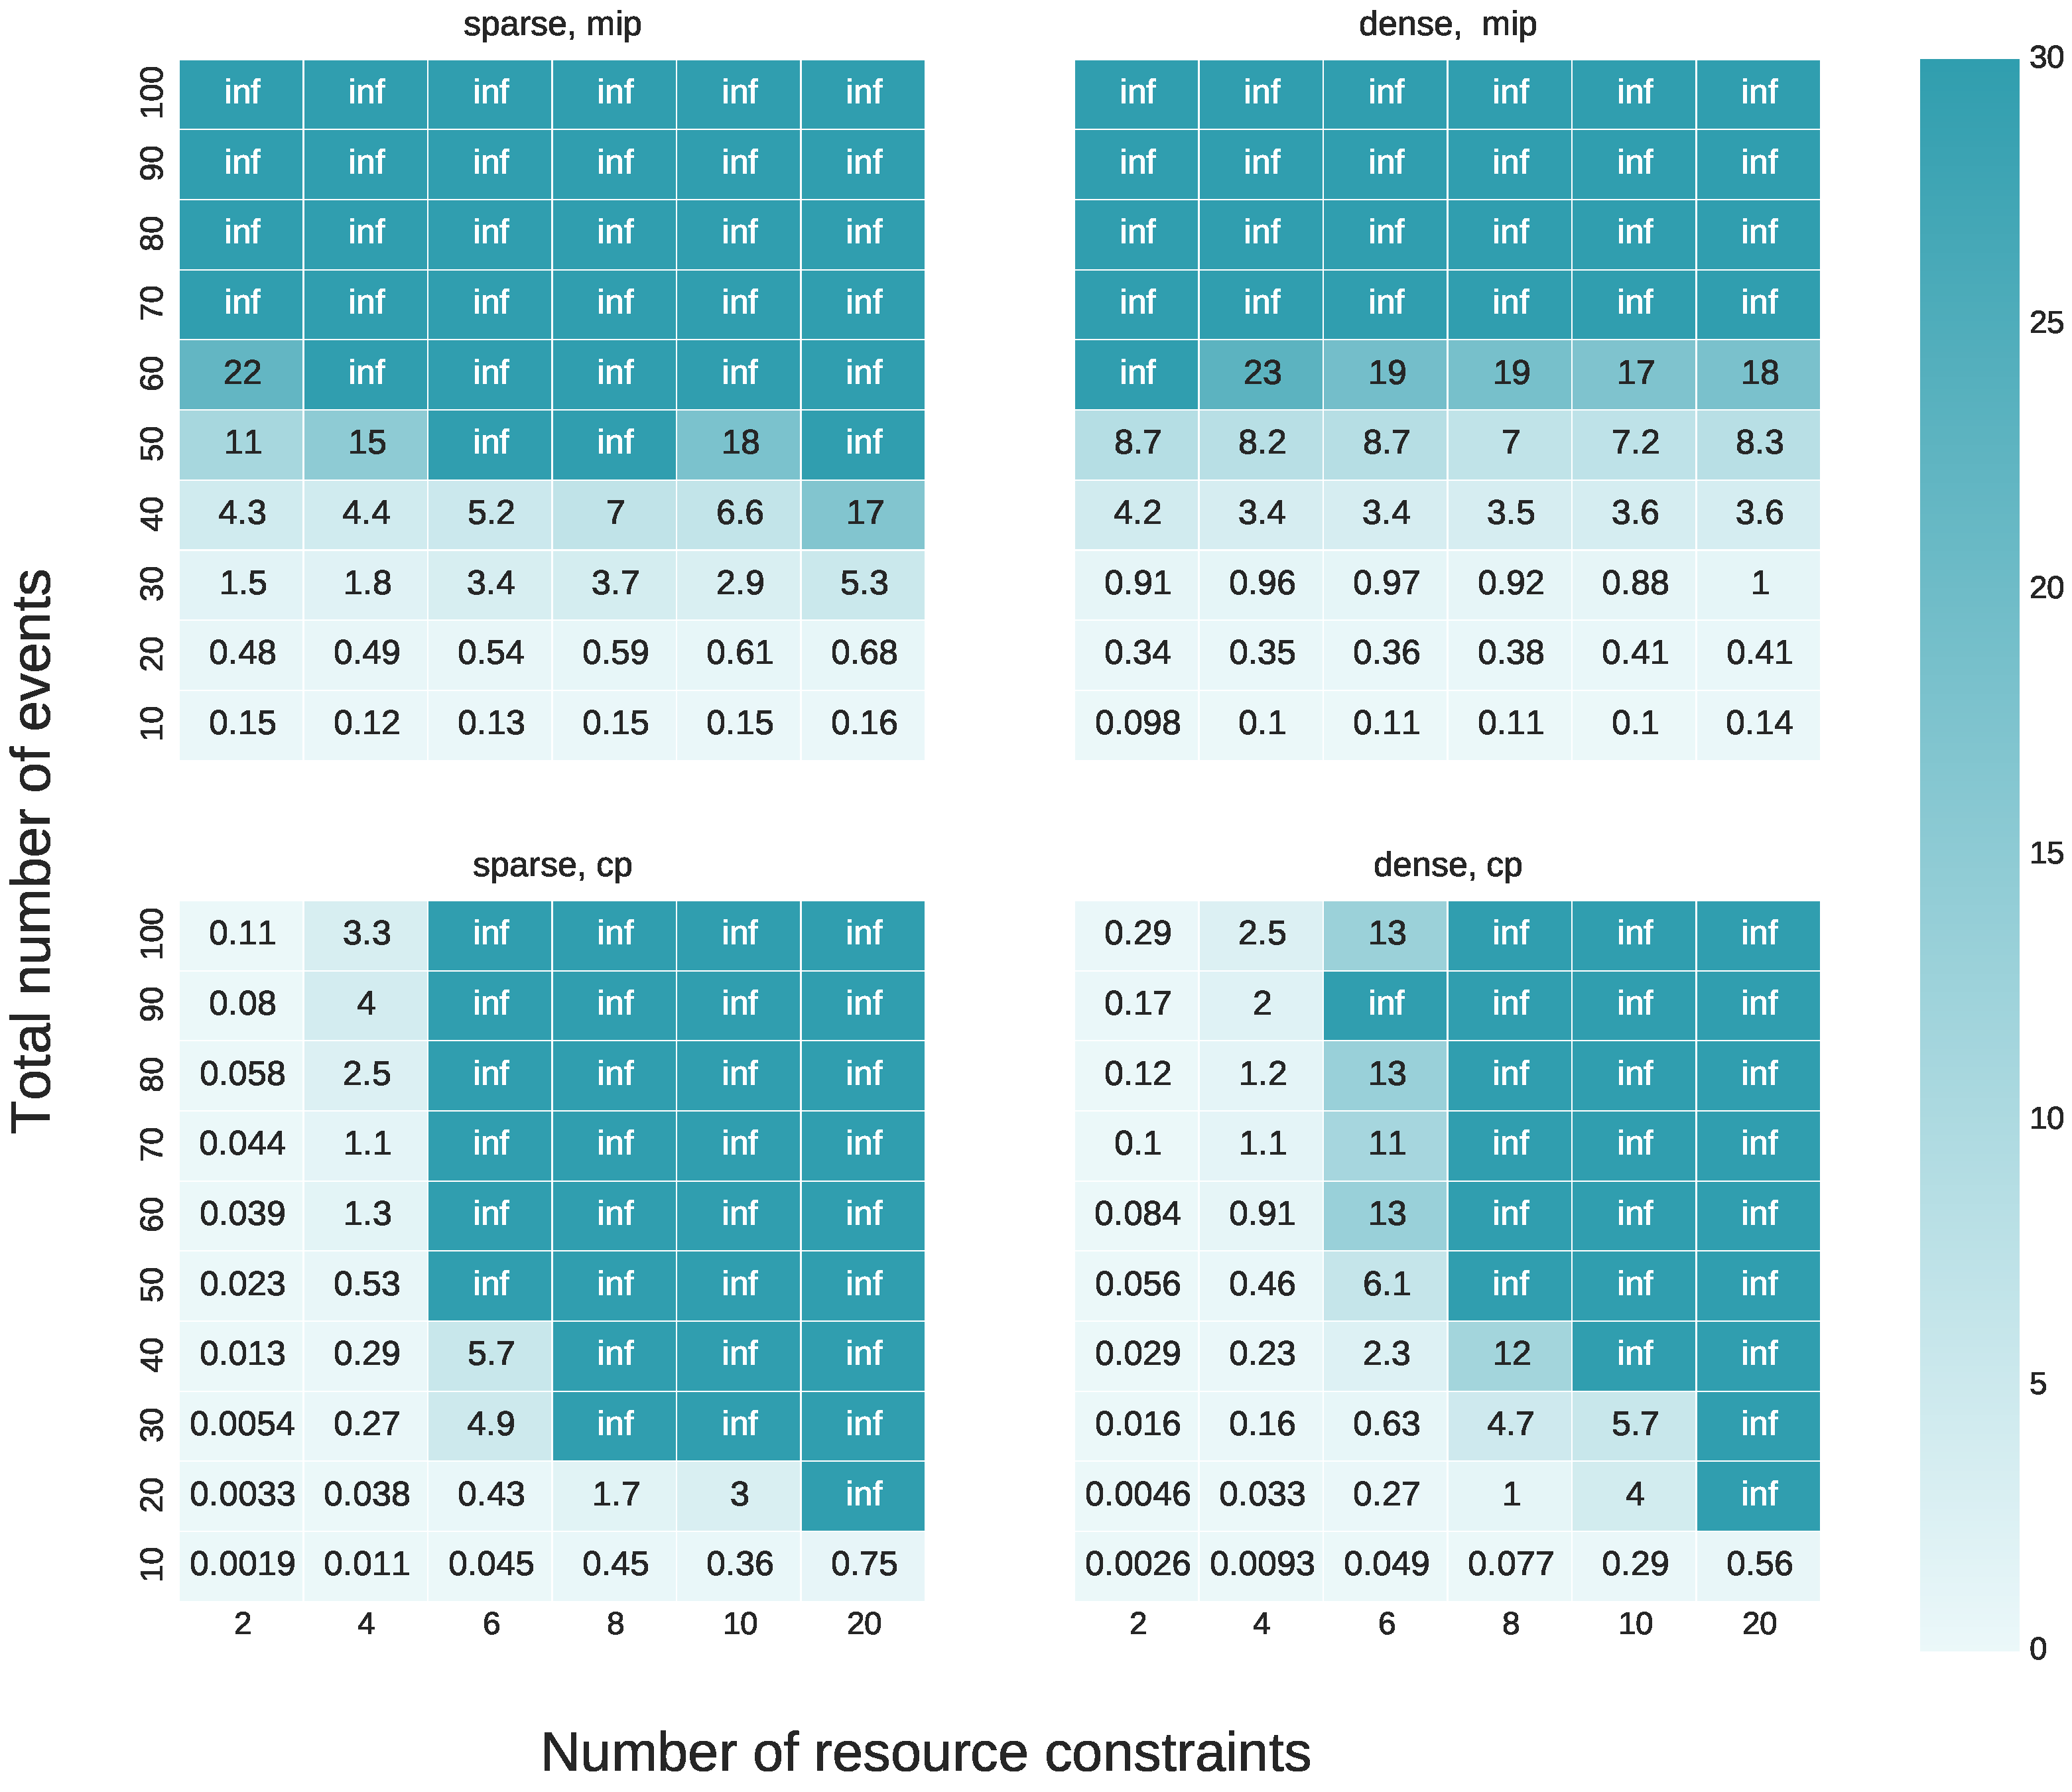
\includegraphics[width=\textwidth]{../execution_time}
\caption{Comporison of execution time for different types of networks, or \texttt{inf} if the solver failed to compute the result within time limit. Y axis represents the number of nodes in the temporal network ($N$). X axis represents the number of resource constraints ($R$). Top portion of the figure was obtained using the MIP-based solver, while bottom part of the figure was obtained using CP-based solver. The left side of the figure represents computations on \textit{sparse} networks, which in this case means that the total number of temporal constraints is $2N$. On the right side we have \textit{dense} networks, meaning that the number of temporal constraints is $N^2/2$.}
\label{fig:execution_time}
\end{center}
\end{figure*}

\begin{figure*}
\begin{center}
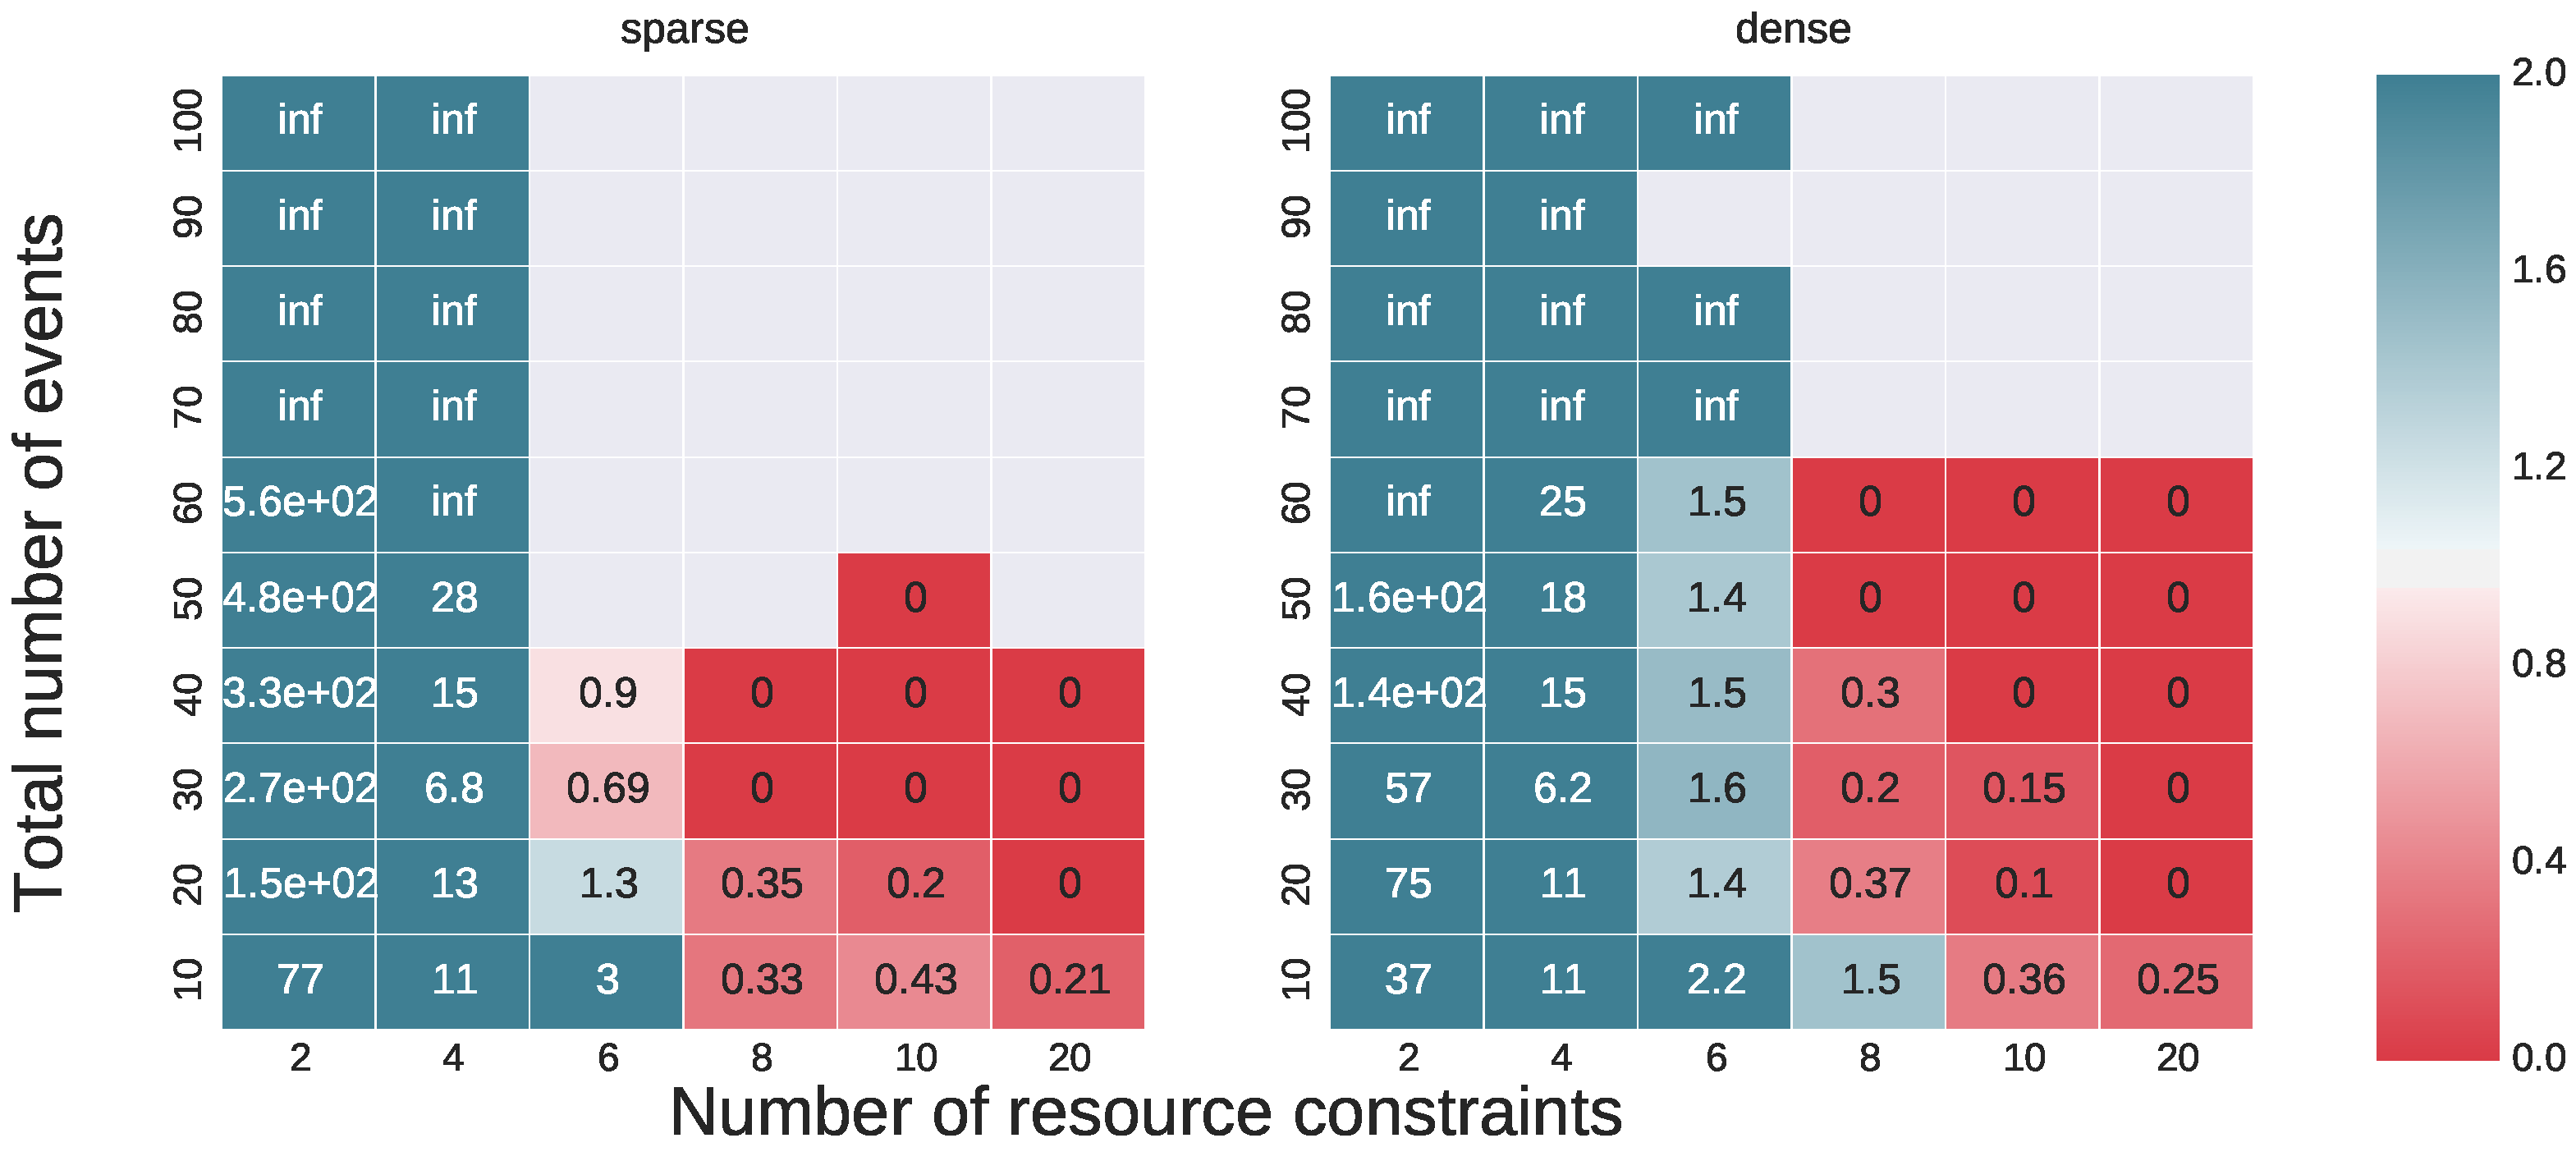
\includegraphics[width=\textwidth]{../when_better}
\caption{Number on the figure represents execution time using CP-based algorithm divided by execution time using MIP-based algorithm. Notice that in particular $0$, means that MIP-based algorithm failed to compute the results within the time limit and \texttt{inf} means that CP-based algorithm timed out. The missing cells correspond to the networks where both of the algorithms timed out and therefore their execution time cannot be compared.   }
\label{fig:when_better}
\end{center}
\end{figure*}


\subsection{TRN over pSTN}
To demonstrate extensibility of our approach we have implemented a version of TRN network, where the underlying temporal network is pSTN (\cite{Fang2014}). pSTN extends the notion of STN. For this discussion we define STN nodes and edges as \textbf{actiavated time points} and \textbf{free constraints} respectively. pSTN defines \textbf{received time point} which is determined by the environment. Every received time point is defined by corresponding \textbf{uncertain duration (uDn)} constraint, which specifies a probability distribution over duration between an activated time point and a received time point. Due to that extension, the notion of consistency becomes probabilistic; rather than asking \textit{is this pSTN consistent?}, we ask is \textit{is this pSTN consistent with probability $p$?}. Since pSTN is an extension of STN, it is an ATN.

Let's consider the following Smart House scenario. We have $150W$ generator which is available. We know that the user comes back from work at some time defined by a gaussian distribution $N(5pm, 5m)$. Moreover we know that sun sets at time defined by $N(7pm, 1m)$. We would like to meet the following constraints with the overall probability at least $98\%$:
\begin{itemize}
\item Wash clothes (duration: $2h$, power usage: $130W$) before user comes back from work
\item Cook dinner (duration: $30m$, power usage: $100W$) ready within 15 minutes of user coming back from work
\item Have the lights on (power usage: $80W$) from before sunset to at least midnight.
\item Cook a late night snack (duration: $30m$, power usage: $20W$) between 10pm and 11pm.
\end{itemize}


\begin{figure}[H]
\begin{center}
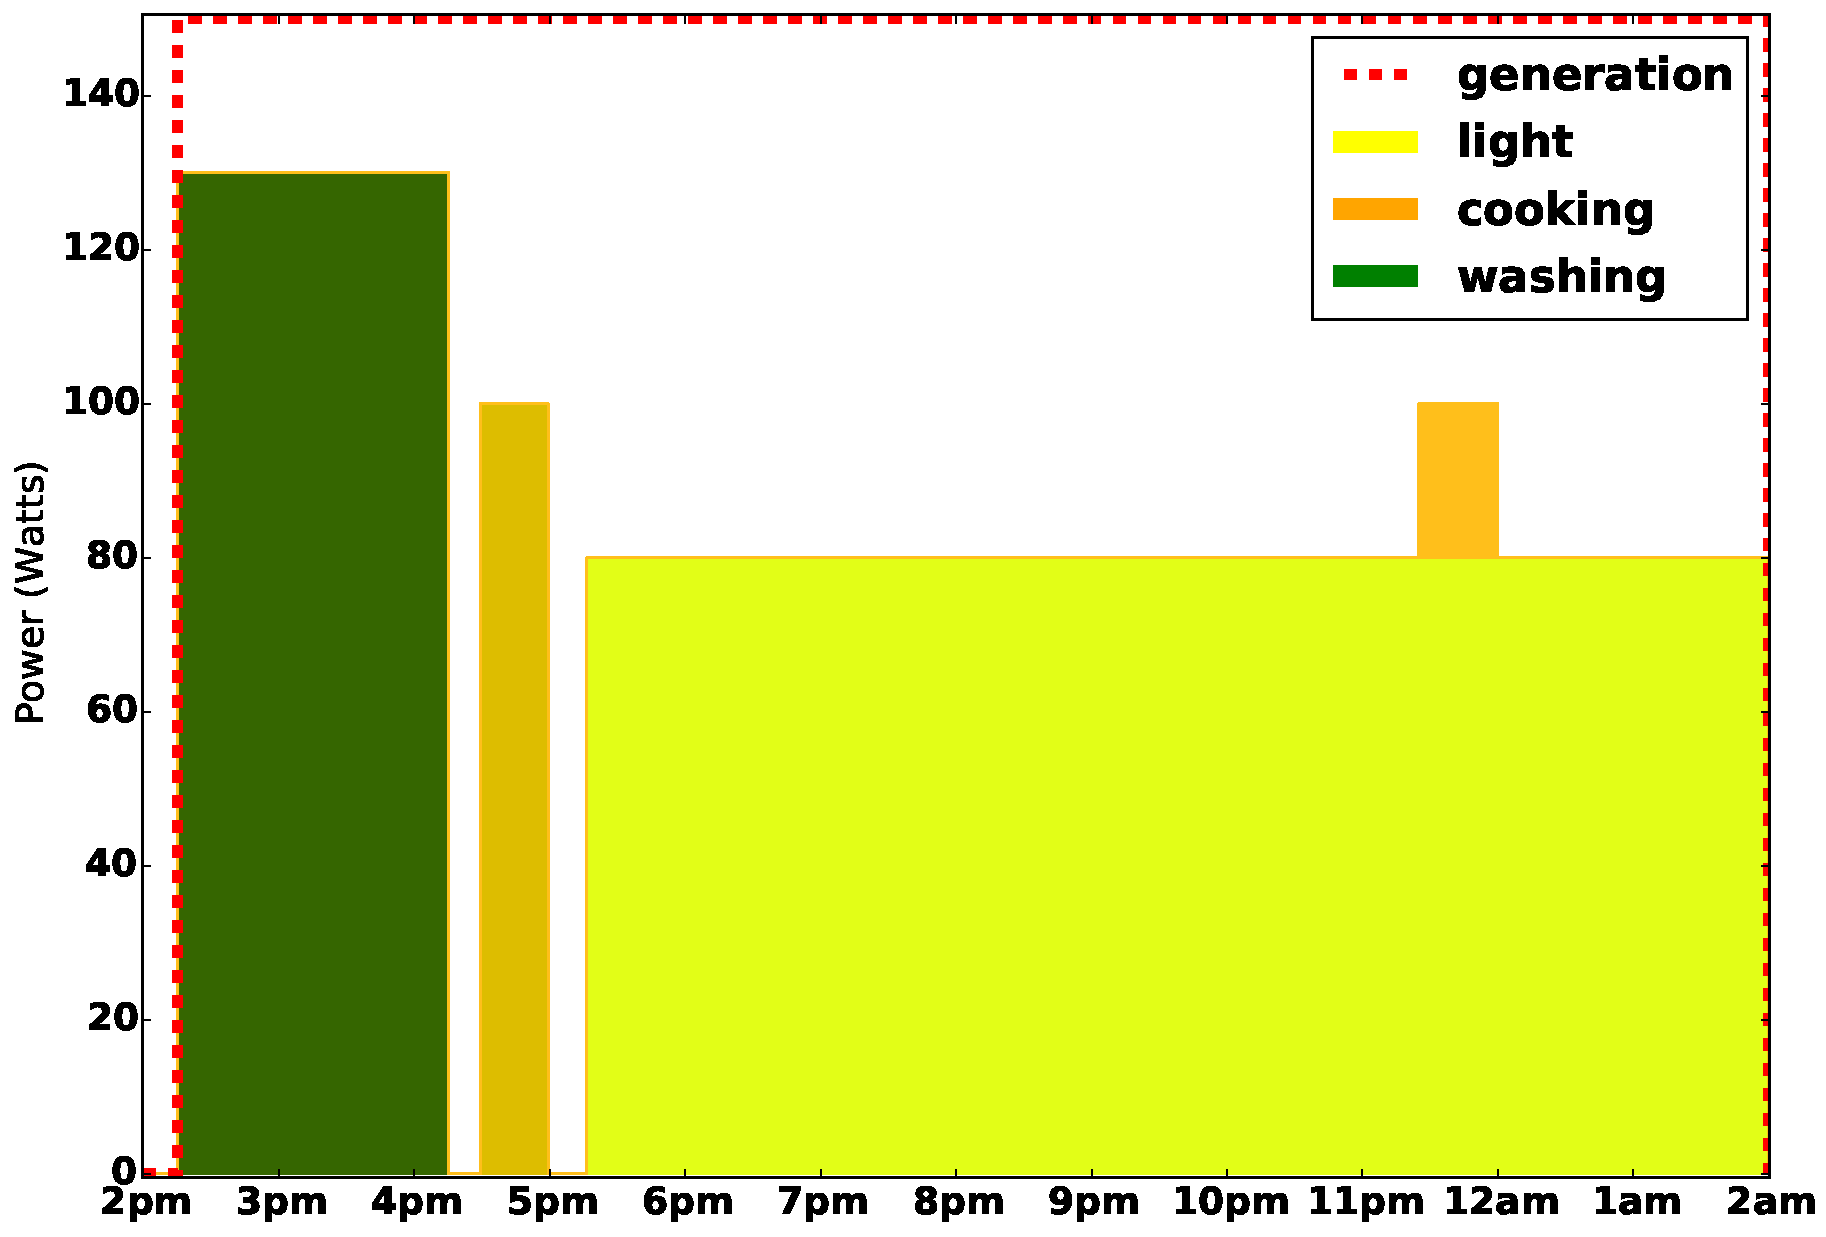
\includegraphics[width=0.49\textwidth]{../pstnu_scheduling}
\caption{Depiction of solution to TRN spanning a pSTN.}
\label{fig:pstnu_scheduling}
\end{center}
\end{figure}

Our algorithm successfully finds a solution to this scenario which meets the constraints with probability $99,7\%$, which is more than required. It is presented on fig. \ref{fig:pstnu_scheduling}.



%%%%%%%%%%%%%%%%%%%%%%%%%%%%%% FUTURE WORK %%%%%%%%%%%%%%%%%%%%%%%%%%%%%%%%%%%%
\section{Future Work}
\textbf{linear resource constraint} is a triplet $(x, y, r_b, r_e)$, where $x, y \in \texttt{nodes(ATN)}$ and resource usage at time $s(x) \leq t \leq s(y)$ is equal to
\[
    u(t) = r_b + t  \frac{r_e - r_b}{s(y) - s(x)}
\]
Intuitively, simple resource constraint encodes the fact that between time $s(x)$ and $s(y)$  resource is consumed/generated with rate that changes linearly between $s(x)$ and $s(y)$.

\textbf{probabilistic simple resource constraint}
Is an extension of simple resource constraint where $r$ is a random variable (and therefore so is $u(t)$).




%%%%%%%%%%%%%%%%%%%%%%%%%%%%%% CONCLUSION %%%%%%%%%%%%%%%%%%%%%%%%%%%%%%%%%%%%%
\section{Conclusion}
TODO
%%%%%%%%%%%%%%%%%%%%%%%%%%%%%% CONCLUSION %%%%%%%%%%%%%%%%%%%%%%%%%%%%%%%%%%%%%
\section{Acknowledgements}
I would like to thank Peng Yu for useful discussions on my overall approach and support. I would like to thank Cheng Fang for helping me understand pSTNs.

%%%%%%%%%%%%%%%%%%%%%%%%%%%%%% REFERENCES %%%%%%%%%%%%%%%%%%%%%%%%%%%%%%%%%%%%%
\section{References}

\bibliography{references}
\section*{Appendix A}
Figure \ref{fig:execution_time} was computed by running the experiment for every set of parameters multiple times. Figure \ref{fig:std} shows the corresponding standard deviations that can be helpful when judging relevance of results.
\begin{figure*}
\begin{center}
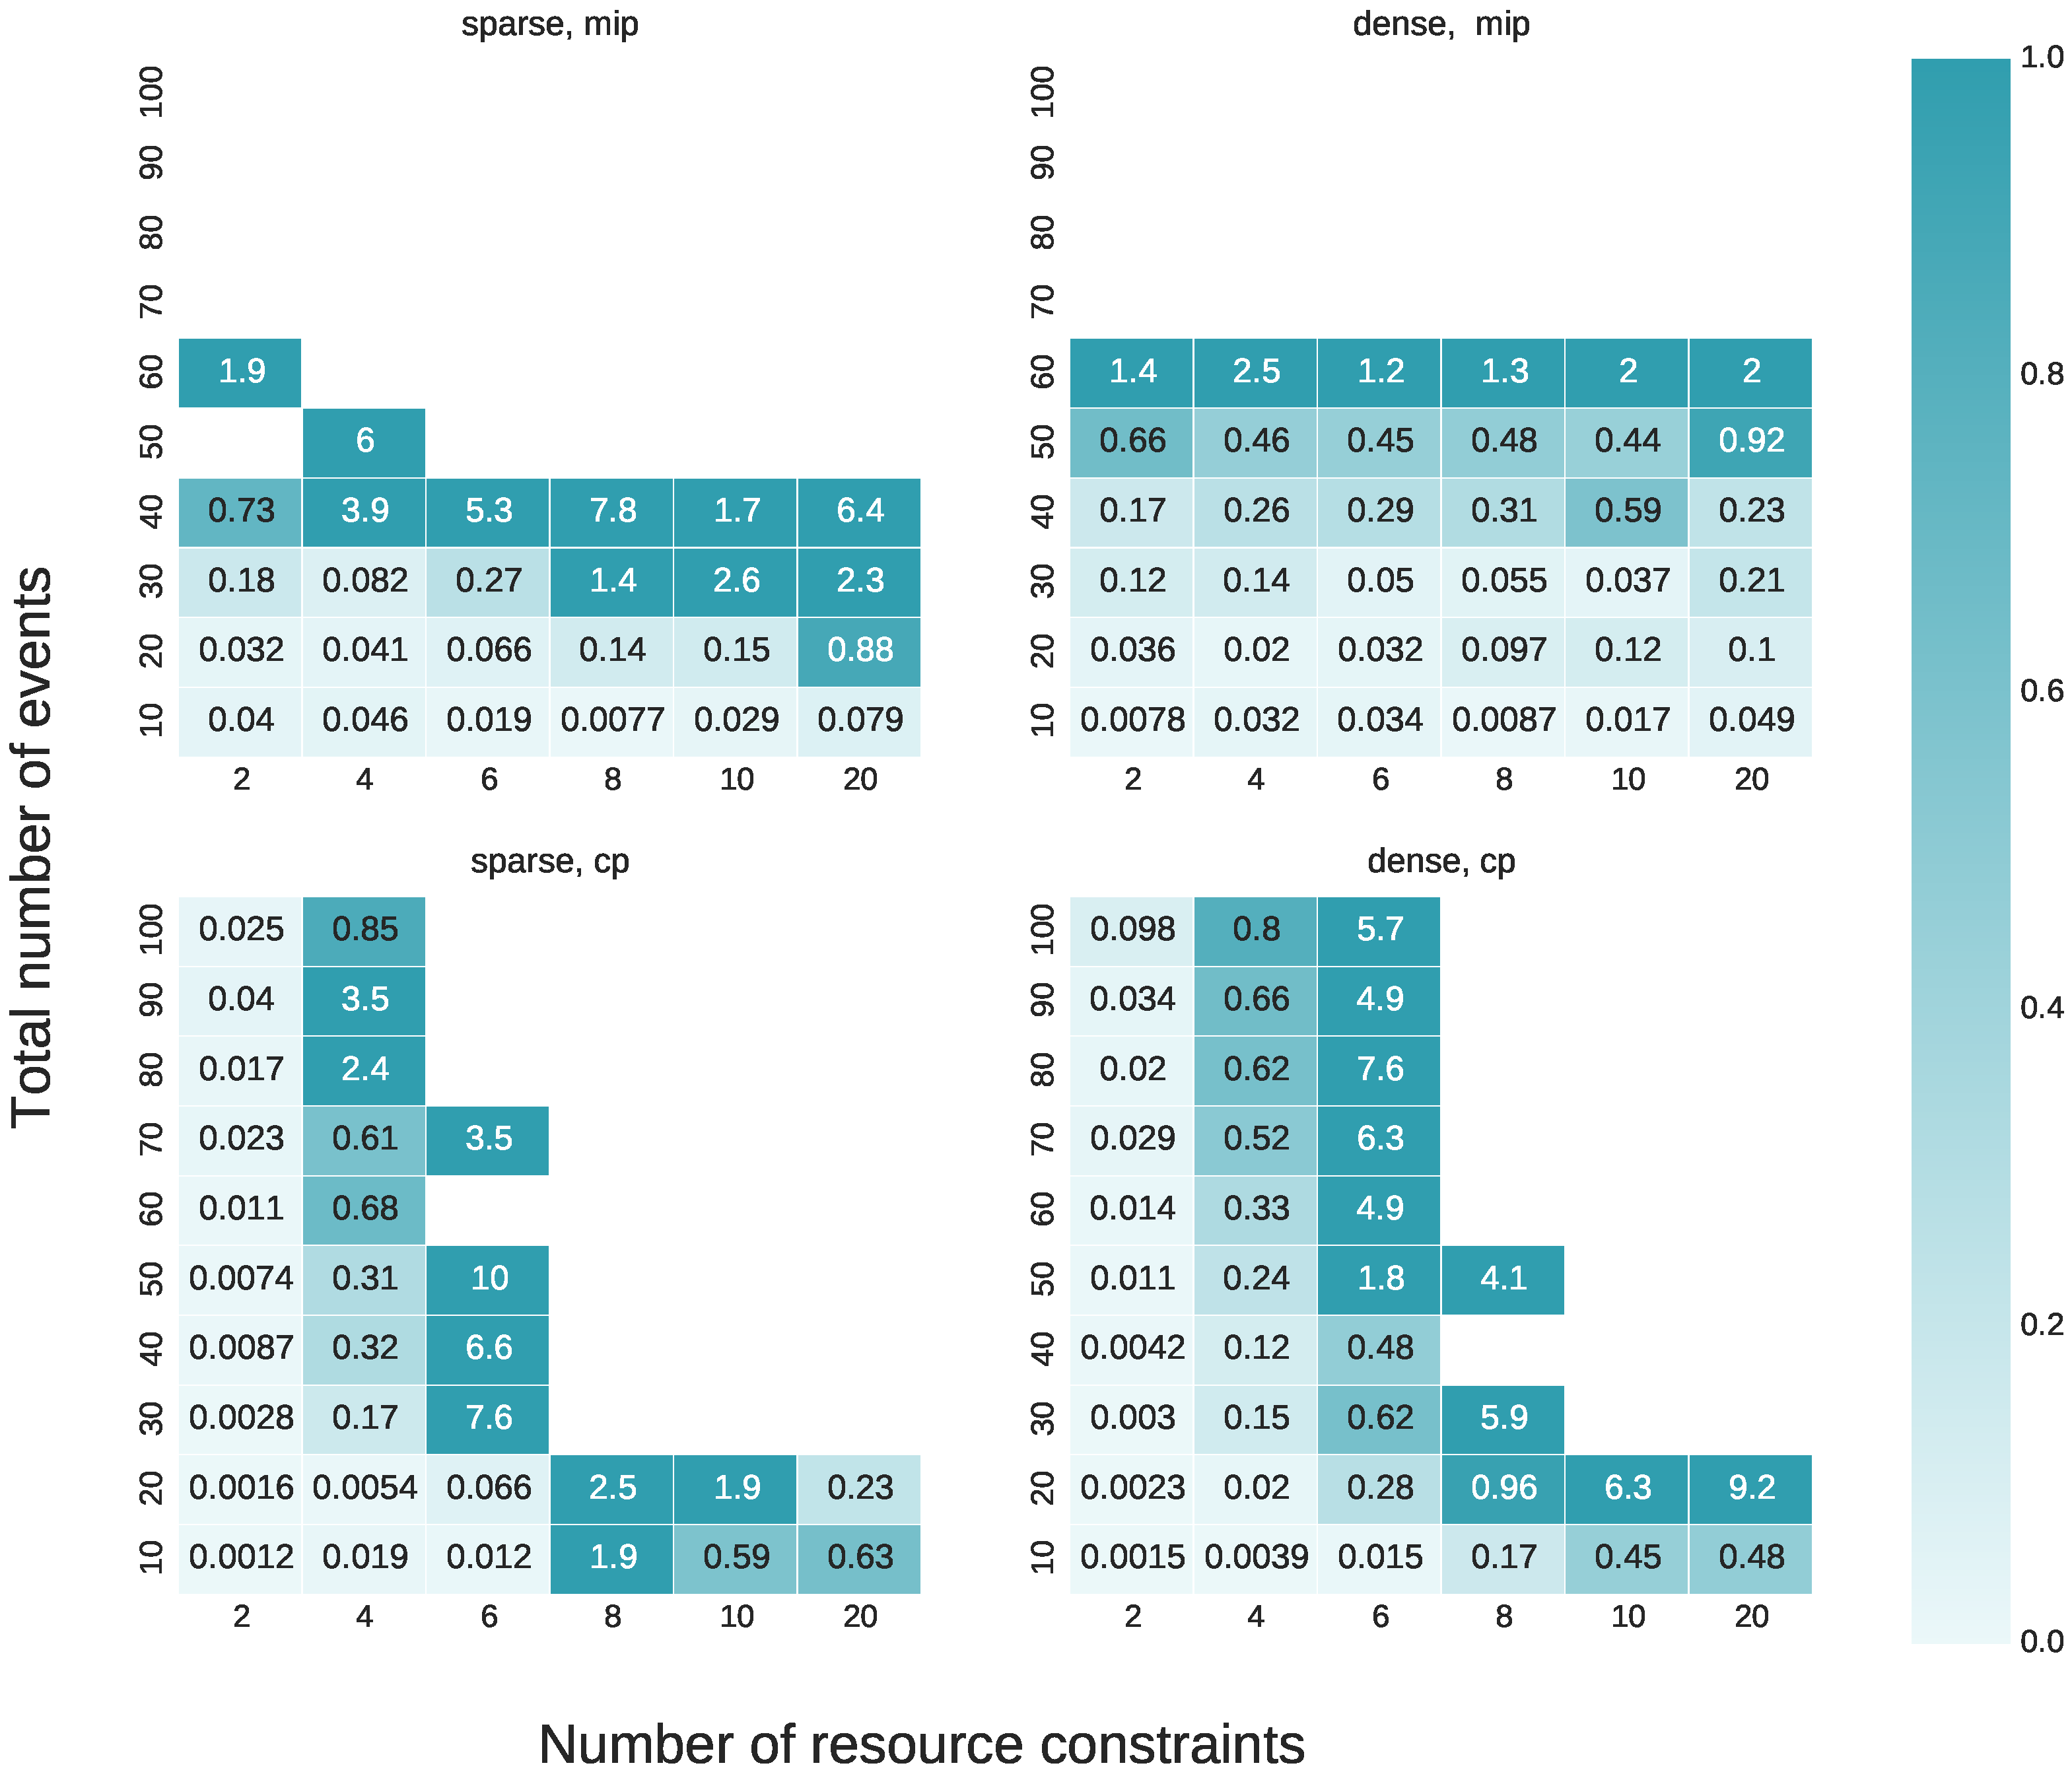
\includegraphics[width=\textwidth]{../std}
\caption{A standard deviation of results from figure \ref{fig:execution_time}. They are laid out in the same way as on that figure.}
\label{fig:std}
\end{center}
\end{figure*}
\end{multicols}
\end{document}
